\tikzset{every picture/.style={line width=0.75pt}} %set default line width to 0.75pt

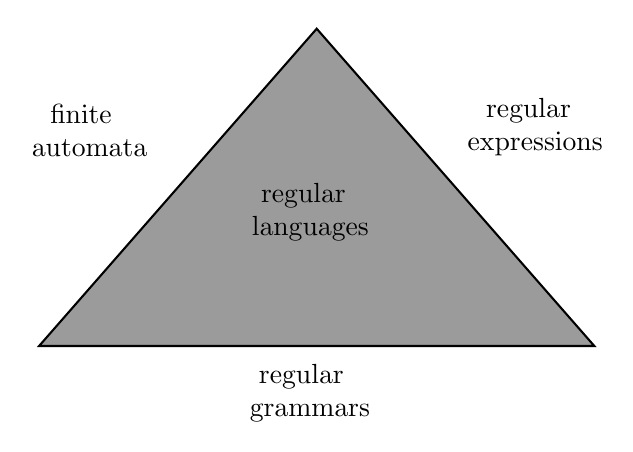
\begin{tikzpicture}[x=0.75pt,y=0.75pt,yscale=-1,xscale=1]
%uncomment if require: \path (0,777); %set diagram left start at 0, and has height of 777

%Shape: Triangle [id:dp3679553887605198]
\draw  [fill={rgb, 255:red, 155; green, 155; blue, 155 }  ,fill opacity=1 ] (152.75,10) -- (286.5,162.86) -- (19,162.86) -- cycle ;

% Text Node
\draw (120,83) node [anchor=north west][inner sep=0.75pt]   [align=left] { \ regular\\languages};
% Text Node
\draw (14,45) node [anchor=north west][inner sep=0.75pt]   [align=left] { \ \ finite\\automata};
% Text Node
\draw (224,42) node [anchor=north west][inner sep=0.75pt]   [align=left] { \ \ regular\\expressions};
% Text Node
\draw (119,170) node [anchor=north west][inner sep=0.75pt]   [align=left] { \ regular\\grammars};
\end{tikzpicture}
